\newpage
\appendix
 
\part*{Appendix}
\addcontentsline{toc}{part}{Appendix}
\section{Matrix Definitions and Theorems}
\subsection{Norms}
A \emph{norm} is a function $\norm{\circ}: V \mapsto \R$ quantifying the size of a vector. It must satisfy
\begin{itemize}
    \item \emph{Positive scalability:}
    \begin{align*}
        \norm{a\cdot x} &= |a|\cdot \norm{x}.
    \end{align*}
    \item \emph{Triangle inequality}
    \begin{align*}
        \norm{x+y} \leq \norm{x} + \norm{y} \quad \forall x,y \in V.
    \end{align*}
    \item \emph{Separability}:
    \begin{align*}
        \norm{x} = 0 \ \implies \ x=0.
    \end{align*}
\end{itemize}
\subsubsection{Vector norms}
\begin{description}
    \item[$\mathbf{p}$-norms] The most commonly used matrix norms are $p$-norms.
        \begin{align*}
            \norm{x}_p := \left(\sum_{i-1}^n |x_i|^p\right)^{1/p}
        \end{align*}
        for $p \in [1,\infty]$, where $|x_i|$ denotes the absolute value of coordinate $x_i$.
        
        A special case of the $p$ norm is the \emph{Eclidean norm}:
        \begin{align*}
            \norm{x}_2:= \sqrt{\sum_{i=1}^n x_i^2}.
        \end{align*}
    \item[$0$-norm] technically not really a norm is defined by:
        \begin{align*}
            \norm{x}_0 := \text{number of nonzero coordinates in $x$}.
        \end{align*}
\end{description}
\subsubsection{Matrix norms}
\begin{description}
    \item[$p$-norm] for matrices:
        \begin{align*}
            \norm{X}_p := \max_{x\neq 0} {\norm{Ax}_p \over \norm{x}_p}.
        \end{align*}
        A special case is the Euclidean or \emph{spectral norm}:
        \begin{align*}
            \norm{X}_2 = \sigma_\text{max} (X),
        \end{align*}
        the largest singular value of $X$.
    \item[Frobenius norm] is defined as:
        \begin{align*}
            \norm{X}_F := \sqrt{\sum_{i=1}^m \sum_{j=1}^n x_{ij}^2} = \sum_{i=1}^{\text{min}(m,n)} \sigma_i^2,
        \end{align*}
        where $\sigma_i$ are the singular values of $X$.
        
        
\end{description}

\subsection{Orthogonality}
\begin{description}
    \item[Orthogonal vectors] Two vectors in an inner product are orthogonal if their inner product is zero.
    \item[Orthonormal vectors] Orthogonal vectors that have unit length 1
    \item[Orthogonal matrix] An orthogonal matrix is a square matrix with real entries whose columns and rows are orthogonal unit vectors (i.e. orthonormal vectors).
    For orthogonal matrices it also holds that
    \begin{align*}
        A^T A= I \quad \implies \quad A^T = A^{-1}\ &\text{since,}\\
        (A^TA)_{i,j} &= a_i^Ta_j = 
            \begin{cases}
                1&i=j\\
                0&i\neq j
            \end{cases}
    \end{align*}

\end{description}

\section{Occam's Razor}
\begin{quotation}
Entities must not be multiplied beyond necessity.\end{quotation}
 It states that among competing hypotheses, the hypothesis with the fewest assumptions should be selected. It is often understood as 'the simplest explanation is usually the correct one', although this is potentially misleading.
The application of the principle often shifts the burden of proof in a discussion.[a] The razor states that one should proceed to simpler theories until simplicity can be traded for greater explanatory power. The simplest available theory need not be most accurate. Philosophers also point out that the exact meaning of simplest may be nuanced.\footnote{\url{http://en.wikipedia.org/wiki/Occam's_razor}}

\section{Probability}
We denote $\Omega$ the sample space and by $A$ an event, which is a subset of $\Omega$.
\begin{description}
\item[Probability distribution] A function $p$ that assigns a real number $p(A)$ to each event $A$ is a \emph{probability distribution} if it satisfies the following three axioms:
    \begin{itemize}
    \item $p(A) \geq 0$ for every $A$.
    \item $p(\Omega) = 1$.
    \item If $A_1$, $A_2$, $\ldots$ are disjoint then
        \begin{align*}
            p\left( \bigcup_{i=1}^\infty \right) = \sum_{i=1}^\infty p(A_i)
        \end{align*}
    \end{itemize}
\item[Random Variable] A random variable is a mapping:
    \begin{align*}
        X\ :\ \Omega\ &\rightarrow \ \mathcal K\\
        \omega\ &\mapsto \ X(\omega)
    \end{align*}
    that assigns an element $X(\omega) \in \mathcal K$ to each outcome $\omega$.
    
    Notation and types of random variables (sample spaces):
    \begin{description}
        \item[Notation]:
            \begin{align*}
                X &\quad \text{Random variable}\\
                x &\quad \text{a value taken by the r.v. $X$.}
            \end{align*}
        \item[Discrete random variables]:
            \begin{itemize}
                \item Finite: e.g. $X\in \mathcal B \equiv \{0,1\}$ or $X\in \mathcal S_n$ (set of permutations)
                \item Contably Infinite: e.g $X\in \N,\Z$ etc...
            \end{itemize}
        \item[Continous random variables]: e.g $X\in \R, [a,b]$ etc...

    \end{description}
\end{description}

\subsection{Distributions}
\subsubsection{Categorical distribution}
Multinomial distribution.
\paragraph{Example}
The sample space of throwing two dice is $\Omega = [1,\ldots,6]\times [1,\ldots, 6]$. We consider the two random variables $X_1+X_2$ given by summing up the numbers $x_1, x_2$ of the two dice. The random variable can thus take values in $[2,\ldots, 12]$. This leads to the following probabilites:
\begin{figure}[H]
    \centering
    \begin{tabular}{r|ccccc ccccc c}
        Random variable &2&3&4&5&6&7&8&9&10&11&12\\\hline
        Probability & ${1\over 36}$& ${2\over 36}$& ${3\over 36}$&  ${4\over 36}$& ${5\over 36}$&  ${6\over 36}$& ${5\over 36}$& ${4\over 36}$& ${3\over 36}$& ${2\over 36}$&  ${1\over 36}$
    \end{tabular}
\end{figure}
The random variable $X_1+X_2$ is an example of the \emph{categorical distribution}: A discrete distribution over $K$ events. Each event has the probability $\pi_k$ of occurring.

\paragraph{Definition}
The categorical distribution is a discrete probability distribution whose sample space is the set of $1-$of$-K$ encoded random vectors $x$ of dimensions $K$ having the property:
\begin{align*}
    \sum_{k=1}^K z_k =1, \quad z_k \in \{0,1\}.
\end{align*}
The probability mass function is defined as
\begin{align*}
    p(z| \pi) = \prod_{k=1}^K \pi_k^{z_k},
\end{align*}
where $\pi_k$ represents the probability of seeing element $k$ ($\pi_k \geq 0$, $\sum_{k=1}^K \pi_k =1$).


\subsubsection{Gaussian Distribution}
The probability density function of the Gaussian distribution is given by:
\begin{align*}
    p(x|\mu, \sigma) &= \mathcal N(x|\mu, \sigma) = {1\over \sqrt{2\pi} \sigma} exp \left\{ - {(x-\mu)^2 \over 2\sigma^2 }\right\}\\
    \mu &= \text{ mean of distribution}\\
    \sigma^2 &= \text{ variance of distribution}.
\end{align*}
Probability for $X\in [a,b]$ is given by an integral:
\begin{align*}
    P(a<X<b) = \int_a^b p(x) dx = {1\over \sqrt{2\pi}\sigma} \int_a^b exp \left\{ - {(x-\mu)^2 \over 2\sigma^2 }\right\} dx.
\end{align*}

\subsubsection{Multivariate Gaussian Distribution}
Generalises the univaraite Gaussian distribution to higher dimensions. The distribution samples the space $\mathcal X \subseteq \R^D$. A random vector $X=(X_1, \ldots, X_D)^T$ has a multivariate normal distribution if every linear combination of its components (i.e., $Y=a_1X_1+\ldots+ a_DX_D$) has a univariate normal distribution.

\paragraph{Definition}:
\begin{align*}
    p(x|\mu\Sigma) = \mathcal N(x|\mu, \Sigma) := {1\over (\sqrt{2\pi})^D |\Sigma|^{1/2} } exp \left( -{1\over 2} (x-\mu)^T \Sigma^{-1} (x-\mu)\right)
\end{align*}

\subsubsection{Multidimensional Moment Statistics}
\begin{description}
\item[Expectation] Vector of component expectations:
    \begin{align*}
        \mathbb E[X] = \begin{pmatrix}
                         \mathbb E[X_1]\\
                         \vdots\\
                         \mathbb E[X_D]
                       \end{pmatrix}
    \end{align*}
\item[Variance] Generalised covariance:
    \begin{align*}
        Cov[X,Y] :&= \int_{\mathcal X}\int_{\mathcal Y} p(x,y)(x-\mu_X)(y-\mu_Y) dxdy \\ 
        &=\mathbb E_{X,Y} [(x-\mu_X)(y-\mu_Y)]
    \end{align*}
\item[Covariance Matrix] For random variables $X_1, \ldots, X_D$ we record covariances in the covariance matrix $\Sigma$:
    \begin{align*}
        \Sigma_{i,j} := Cov[X_i,Y_i]\quad i,j \in \{1,\ldots, D\}.
    \end{align*}
    $\Sigma$ generalises the notion of variance to sets of random variables for multiple dimensions.

\end{description}

\subsection{Latent Variables}
Define a $K$-dimensional binary random variable $z$ having a $1$-of-$K$ representation in which a particular element $z_k$ is equal to $1$  and all other elements are equal to $0$, i.e.:
\begin{align*}
    z_k\in \{0,1\}, \qquad \sum_k z_k = 1.
\end{align*}
The marginal distribution over $z$ is specified in terms of the mixing coefficients $\pi_k$, i.e.
\begin{align*}
    p(z_k=1) = \pi_k.
\end{align*}


Because $z$ uses a $1$-of-$K$ representation, we can write this distribution in the form:
\begin{align*}
    p(z) = \prod_{k=1}^K \pi_k^{z_k}.
\end{align*}
Similarly, the conditional distribution of $x$ given a particular value for $z$ is a gaussian:
\begin{align*}
    p(x|z_k=1) = \normal(x|\mu_k, \Sigma_k)^{z_k}.
\end{align*}
The conditional distribution can also be written in the form
\begin{align*}
    p(x|z) = \prod_{k=1}^K \normal(x|\mu_k, \Sigma_k)^{z_k}.
\end{align*}

The marginal distribution of $x$ is obtained by summing the joint distribution over all possible states of $z$ to yield:
\begin{align*}
    p(x) = \sum_z p(z)p(x|z) = \sum_{k=1}^K \pi_k \normal(x|\mu_k, \Sigma_k).
\end{align*}
For the full data log-likelihood we get:
\begin{align*}
    \log p(X|\pi, \mu, \Sigma) = \sum_{n=1}^N \log \left\{\sum_{k=1}^K \pi_k \normal(x_n|\mu_k, \Sigma_k)\right\}.
\end{align*}

\subsection{Bayes' rule}
The conditional probability of $A$ given $B$ (posterior) is given by:
\begin{align*}
    p(A|B) = {p(B|A)p(A)\over p(B)}.
\end{align*}
We call $p(A)$ prior, $p(B|A)$ likelihood and $p(B)$ evidence.


\section{Lagrange Multipliers}
This part was taken from Wikipedia\footnote{\url{http://en.wikipedia.org/wiki/Lagrangian_multiplier}}.

In mathematical optimisation the method of Lagrange multipliers is a strategy for finding the local maxima and minima of a function subject to \emph{equality constraints}.

Consider the two-dimensional problem:
\begin{align*}
    \text{maximise } &f(x,y)&\\
    \text{subject to } &g(x,y)=c,
\end{align*}
with both $f$ and $g$ to having \emph{continuous first partial derivatives}. 


We can visualise contours of $f$ given by
\begin{align*}
    f(x,y) = d,
\end{align*}
for various values of $d$, and the contour of $g$ given by
\begin{align*}
    g(x,y) = c.
\end{align*}
Suppose we walk along the contour line $g=c$. In general the contour lines of $f$ and $g$ may be distinct, so following the contour line for $g=c$ one could intersect with or cross the contour lines of $f$.
Only when the contour line for $g=c$ meets contour lines of $f$ \emph{tangentially}, do we not increase or decrease the value of $f$ (in terms of maximising $f(x,y)$ subject to $g(x,y)=c$).  

The contour lines of $f$ and $g$ touch when the \emph{tangent vectors} of the contour lines are parallel.  Thus we want points $(x,y)$ where $g(x,y)=c$ and
\begin{align*}
    \nabla_{x,y} f= -\lambda \nabla_{x,y} g.
\end{align*}
To solve this system we introduce an auxiliary function:
\begin{align*}
    \Lambda(x,y,\lambda) = f(x,y)+\lambda\cdot (g(x,y)-c),
\end{align*}
and solve
\begin{align*}
    \nabla_{x,y,\lambda} \Lambda(x,y,\lambda) = 0.
\end{align*}

\section{Convex Set}
A set $C$ is convex if the line segment between any two points in $C$ lies in $C$, i.e., if for any $x1,x2 \in C$ and any $\theta$ with $0 \leq \theta\leq 1$, we have
\begin{align*}
    \theta x_1 + (1-\theta)x_2 \in C.
\end{align*}
\begin{figure}[H]
\centering
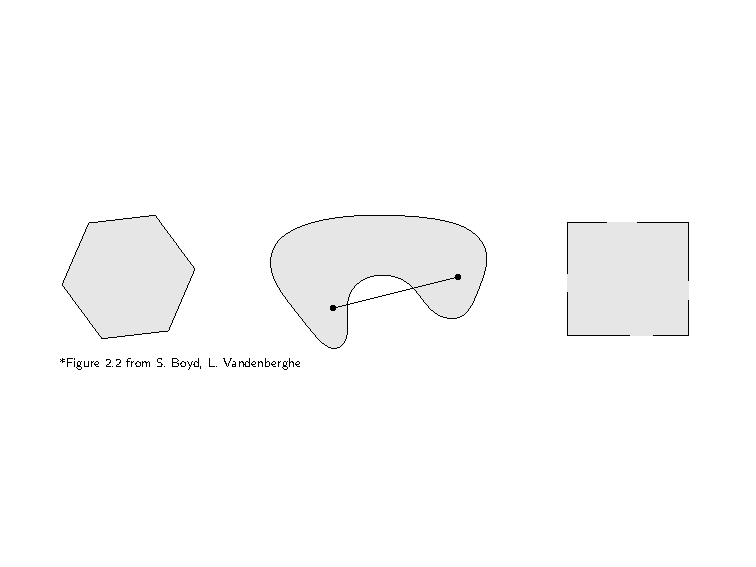
\includegraphics[width=0.8\textwidth]{img/convex_set}
\end{figure}
\begin{description}
\item[Left] Convex.
\item[Middle] Not convex, since the line segment is not in the set.
\item[Right] Not convex, since some, but not all boundary points are contained in the set.
\end{description}

\section{Convex Function}
The graph of a function $f:\R^n \rightarrow \R$ is defined as 
\begin{align*}
    \{
        (x,f(x))\ |\ x\in \text{dom}\ f
    \}.
\end{align*}
The \emph{epigraph} of a function $f:\R^n\rightarrow \R$ is defined as
\begin{align*}
    \{
        (x,f(x))\ |\ x\in \text{dom}\ f,\ f(x)\leq t
    \}.
\end{align*}
\begin{figure}[H]
\centering
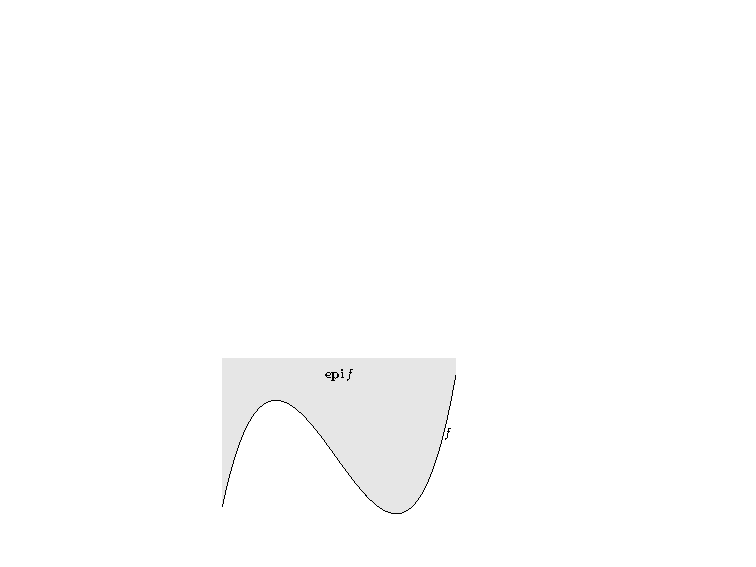
\includegraphics[width=0.4\textwidth]{img/epigraph}
\end{figure}

\paragraph{Examples of convex functions} $\ $
\begin{itemize}
 \item Linear functions: $f(x) = c^T x$
 \item Affine functions: $f(x) = Ax+b$
 \item Exponential: $f(x) = e^{\alpha x}$
 \item Norms Every norm on $\R^n$ is convex.
\end{itemize}

\paragraph{Convexity of a norm $f(x)$} By the triangle inequality 
\begin{align*}
    f(x+y) \leq f(x) + f(y)
\end{align*}
and homogeneity of a norm 
\begin{align*}
    f(\alpha x) &= |\alpha| f(x) &\alpha \text{ a scalar}
\end{align*}
we can prove that:
\begin{align*}
    f(\theta x+(1-\theta)y)\leq f(\theta x)+f((1-\theta)y) = \theta f(x) + (1-\theta)f(y).
\end{align*}








